\Chapter{Az alkalmazás felépítése}

\Section{Felhasznált eszközök és technológiák}

A feladatom webalkalmazás készítése éttermek és rendelések adatainak nyilvántartásához. Ennek megvalósításához a Python programozási nyelvet, és a Flask webes keretrendszert választottam. A felhasználói felület létrehozása webes környezetben, HTML5 és AngularJS segítségével történt. Az adatokat SQLite alapú relációs adatbázisban tárolom, amelyhez a keretrendszer SQLAlchemy ORM-en keresztül csatlakozik. A dolgozatom készítése során a GitHub nevű online verziókövető rendszert használtam.

A következő részekben a felhasznált technológiák választásának okát, fontosabb tudnivalóit és felhasználási módját taglalom.

\SubSection{Git}

A Git jelenleg a világon a legszélesebb körben használt modern verziókezelő rendszer \cite{git}. A Git egy nyílt forráskódú, elosztott verziókezelő rendszer, melyet 2005-ben fejlesztett ki Linus Torvalds, a Linux kernel atyja. Minden Git munkamásolat egy teljes értékű repository teljes verziótörténettel és teljes revíziókövetési lehetőséggel, amely nem függ a hálózat elérésétől vagy központi szervertől. Számos nagy volumenű projekt használja jelenleg a Gitet verziókezelő rendszerként.

\SubSection{GitHub}

A GitHub egy Git alapú verziókövető, és egyben egy ingyenes internetes tárhely \cite{github}. Szolgáltatja az elosztott verziókezelő rendszer és a forráskód-menedzselés minden funkcióját. Biztosítja a hozzáférés-szabályozást és még számos más funkciót, mint például a bug tracking, feature requests, vagy task managment. Ezek tudatában döntöttem a GitHub használata mellett.

\SubSection{Python}

A Pythont Guido van Rossum holland programozó kezdte el fejleszteni 1989 végén \cite{python}. A Python egy széles körben használt, nagyon magas szintű általános célú programozási nyelv. Ez egy úgynevezett interpreteres nyelv, ami azt jelenti, hogy nincs különválasztva a tárgykód és a forráskód. A Python iterpretert számos géptípusra és operációs rendszerre elkészítették. A nyelvnek van egy sajátos tervezési filozófiája, ami az olvashatóságot, és a programozói munka megkönnyítését helyezi előtérbe. Olyan szintaxisa van, amely lehetővé teszi a programozók számára, hogy kevesebb kódsoron fogalmazzák meg a koncepciókat, mint például a C\# vagy a Java nyelvek esetében.

A Python támogatja a dinamikus típusokat és az automatikus memóriakezelést, emellett szigorú típusrendszerrel rendelkezik. Számos programozási paradigmát támogat, mint például az objektumorientált, funkcionális, imperatív vagy procedurális.

\SubSection{Flask}

Miután kiválasztottam a Pythont, szükségem volt még az alkalmazásom elkészítéséhez egy webes keretrendszerre. Számos Python alapú webes keretrendszert találtam, ezek közül hárommal szimpatizáltam. Ez a három a Django, a Flask és a Pyramid volt. Miután összevettem őket, arra a következtetésre jutottam, hogy a feladatom megvalósításához a Flask lesz a legalkalmasabb.

A Flask lényegében egy Python nyelven íródott Werkzeug eszközrendszeren alapuló, Jinja2 template motort használó webes mikro keretrendszer \cite{flask}. A Flaskot azért nevezik mikro keretrendszernek, mert nem igényel speciális eszközöket vagy könyvtárakat. Nem rendelkezik adatbázis-absztrakciós réteggel, form validációval, vagy bármely más olyan összetevővel, ahol már létező, harmadik féltől származó könyvtárak közös funkciókat biztosítanak. Azonban a Flask olyan bővítményeket támogat, melyek képesek alkalmazási funkciók hozzáadására, úgy mintha azok eleve implementálva lettek volna a Flaskban. Bővítmények léteznek az objektum-relációs leképzésre, űrlap validációra, fájlfeltöltés kezelésére és még számos közös keretrendszerhez kapcsolódó eszközre. Ezeknek a bővítményeknek sokkal gyakrabban jön ki friss verziójuk, mint magának a Flasknak.

\SubSection{Pycharm}

A Pycharm a JetBrains által fejlesztett Python integrált fejlesztői környezet \cite{pycharm}. A Pycharm biztosít kód analízist, grafikus debuggert, egy integrált egységtesztelőt, integrációt verzió kezelő rendszerrel, és támogatja a web fejlesztést.

Azért esett erre a fejlesztői környezetre a választásásom, mert korábban már használtam a JetBrains által fejlesztett szoftvereket, és nagyon elégedett voltam velük. Megbízható, stabil, gyors, és nagyon sok alap funkció van bele integrálva, tehát nem kell különféle pluginokat telepítenem, mint például az Eclipse esetében.

\SubSection{HTML5}

A HTML (angolul HyperText Markup Language) egy általános leíró nyelv, melyet weboldalak és webes alkalmazások készítésre használnak \cite{html}. A HTML mára már internetes szabvánnyá vált a W3C (World Wide Web Consortium) támogatásával.

A HTML5 az ötödik és egyben a jelenleg a legjelentősebb verziója a HTML-nek. 2014 októberében publikálta a W3C, a fejlesztés egyik fő célja, hogy a webes alkalmazásokhoz ne kelljen telepíteni a különböző multimédiás plugineket. A HTML5 visszamenőleges kompatibilitást biztosít.

\SubSection{Cascading Style Sheets (CSS)}

A stíluslapok úgynevezett stílusszabályokból állnak, melyeket egy stílusleíró nyelven adunk meg, ez a stílusleíró nyelv a Többszintű Stíluslapok nyelve, azaz a CSS \cite{css}. A CSS segítségével tudjuk leírni a jelölőnyelv alapú (például HTML) strukturált dokumentumok megjelenését. Megadhatjuk az HTML dokumentum minden egyes elemének a stílusát. A stíluslap minden eleme kijelölőből (selector) és meghatározásból (declaration) áll.

\SubSection{Bootstrap}

A Bootstrap egy ingyenes, nyílt forráskódú front-end webes keretrendszer weboldalak és webes alkalmazások megjelenésének tervezésére \cite{bootstrap}. HTML és CSS alapú sablonokat tartalmaz a betűtípusok, formok, gombok, egyéb interfész-összetevők, valamint az opcionális JavaScript-bővítmények számára. A Bootstrap ellentétben más webes keretrendszerekkel, csak front-end fejlesztéssel foglalkozik. A Bootstrap az egyik legnépszerűbb keretrendszer, melyet responsive webes alkalmazások fejlesztésére használnak.

\SubSection{JavaScript}

A JavaScript egy Netscape által fejlesztett, interpreteres programozási nyelv \cite{javascript}. Gyengén típusos, dinamikus nyelv, amely lehetővé teszi dinamikus események kiváltását HTML alapú weboldalakon. Javan alapul, közvetlenül HTML dokumentumba épül be és a webböngésző értelmezi.

\SubSection{AngularJS}

Az AngularJS egy JavaScript alapú nyílt forráskódú front-end webes keretrendszer, melyet főként single-page alkalmazások fejlesztésénél használnak \cite{angularjs}. Az AngularJS felfogható egy MVC keretrendszernek. Model réteg alatt a JavaScript változókat kell érteni, melyek az adatokat tárolják. A view réteg maga a HTML kód, amit az AngularJS további beágyazott egyedi tag attribútumokkal egészít ki. Ezek a beágyazott attribútumok rendelik össze a view réteget a model és controller rétegekkel. A controller réteget a JavaScript függvények adják, amik módosítják a model rétegben lévő JS változókat.

A JavaScript analitikai szolgáltatása, a Libscore szerint az AngularJS-t használja a Wolfram Alpha, NBC, Walgreens, Intel, Sprint, ABC News, valamint a 2016 októberében tesztelt 1 millió weblap közül további 12000. Az AngularJS jelenleg benne van a top 100 legelterjedtebb GitHub projekt között.

\SubSection{Ajax}

Az Ajax (Asynchronous JavaScript And XML) egy kliensoldali webfejlesztési technika, melyet interaktív webalkalmazások létrehozására használunk. Az Ajax lényege, hogy a webalkalmazás a háttérben folyamatosan kis mennyiségű adatot cserél a szerverrel aszinkron módon, anélkül, hogy zavarná a betöltött oldal megjelenítését vagy viselkedését. Ennek hatására nem kell az oldalt újra tölteni minden egyes apró felhasználói módosítás után. Ezzel az Ajax növeli a honlap sebességét, interaktivitását és használhatóságát.

\SubSection{JavaScript Object Notation}

A JSON egy szöveg alapú, kis méretű, nyílt szabvány ember által olvasható adat objektumok cseréjére. Ez egy nagyon elterjedt adatformátum, melyet aszinkron szerver-kliens kommunikációnál használnak az XML helyett. A JSON nyelvfüggetlen, több nyelvhez is van értelmezője.

\SubSection{JSON Web Token}
A JWT egy JSON alapú nyílt szabvány hozzáférési tokenek létrehozásához, melyek néhány követelést tartalmaznak \cite{jwt}. A követelések jellemzően a hitelesített felhasználók identitásának azonosítására szolgálnak. A tokenek hitelesíthetők és titkosíthatók.

\SubSection{SQLAlchemy}

Az SQLAlchemy a Pythonhoz írt nyílt forráskódú ORM rendszer \cite{sqlalchemy}. Széles körű szolgáltatást nyújt adatbázis-függetlenül, kezdve az egyszerű lekérdezés generálástól az átfogó, akár többszörös összekapcsoláson át egészen a táblák alapvető információinak kinyeréséig. Könnyű használhatósága és teljesítménye miatt ez a ma leggyakrabban használt ORM eszköz Python rendszerekhez.

Az SQLAlchemy egyik nagy előnye, hogy képes egyszerre magas és alacsony szintű absztrakciót nyújtani, a rendszer elvárásától függően. A leggyakrabban használt Python keretrendszerek, mint például a Flask vagy a Django, nagy mértékű támogatást nyújtanak hozzá, ennek köszönhetően nagyon fejlesztőbarát megoldásnak tekinthető.

\Section{Az alkalmazás fő részei}

Az alkalmazás szerveroldalon a \textit{Python/Flask} keretrendszert, kliensoldalon pedig \textit{AngularJS}-t használ. Az adatokat relációs adatbázisban tárolom, amelyhez a keretrendszer \textit{SQLAlchemy ORM}-en keresztül csatlakozik. Létrehoztam egy nyilvántartás nevű csomagot, ami alacsonyabb szintű programészre épülve magasabb szintű funkciókat valósít meg, elfedve a technikai részleteket. Az alkalmazás logikai felépítést \aref{fig:architecture1}. ábra szemlélteti.

\begin{figure}
\centering
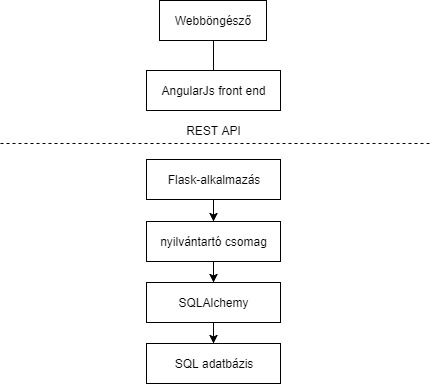
\includegraphics[scale=0.8]{kepek/architecture.jpg}
\caption{A webalkalmazás architektúrája}
\label{fig:architecture1}
\end{figure}

A felhasználó böngészőn keresztül tudja használni az alkalmazást. Az alkalmazás használója ilyenkor az AngularJs-sel kialakított úgynevezett nézeteket látja. Kliens oldalon az Angular kontrollerjei végzik a kérések elküldését a szerver irányába, melyekre a szerver az adatok visszaküldésével válaszol. A kapott válaszokat szintén az kontrollerek dolgozzák fel. A felhasználói felületről és az Angularról az ötödik fejezetben fogok bővebben írni.

% TODO: Apróság, de a fejezetet itt is majd \ref-el kellene hivatkozni!

A szerver oldalon egy többrétegű struktúrát hoztam létre. Az alsó réteg az adatbázis, ami egy SQLite alapú relációs adatbázis, amelyhez a keretrendszer SQLAlchemy ORM-en keresztül csatlakozik, tehát a lekérdezéseket az SQLAlchemy-vel végzem. Az SQL adatbázist a 4. fejezetben fogom részletesebben taglalni.

A klienstől érkező kérések feldolgozására az alkalmazás a Flask webes mikro keretrendszert használja. A flaskos réteg HTTP válaszokat küld a kliensnek, melyeben az adatok JSON formátumúak. A flaskos réteg és az alsóbb rétegek között van egy közbenső réteg, az általam készített nyilvántartó csomag. A nyilvántartó csomagban lévő metódusok végzik a lekérdezéseket, ezeket a metódusokat hívom meg a flaskos rétegben. A közbenső réteg bevezetésére a későbbi továbbfejlesztési lehetőségek miatt volt szükség. A flask és a nyilvántartó csomag bemutatására a ötödik fejezetben fog sor kerülni.

\Section{Az alkalmazás alapfunkciói}

Az alkalmazásom lényegében éttermek és rendelések adatainak nyilvántartására fog szolgálni. Ebben a fejezetben az alap funkcionalitásokat fogom tárgyalni. Az első ezek közül a regisztrációval, bejelentkezéssel, felhasználói adatok kezelésével kapcsolatosak, azt követően pedig a vásárlói és étteremtulajdonos funkciók bemutatása következik.

\bigskip

\noindent \textbf{Regisztráció/bejelentkezés}

\medskip

Az alkalmazásom egyik alap funkcionalitása a felhasználókezelés lesz. Csak regisztrált felhasználók számára lesznek elérhetőek a szolgáltatások, a kezdőlapon lesz lehetőség a bejelentkezésre vagy regisztrációra. Alapvetően két felhasználói csoportot lehet majd megkülönböztetni, a vásárlókat és az étteremtulajdonosokat. A két csoport eltérő jogosultsági körrel fog rendelkezni, és más-más szolgáltatások lesznek számukra elérhetőek.

\bigskip

\noindent \textbf{Felhasználói adatok megjelenítése}

\bigskip

A felhasználók számára lesz egy szolgáltatás, amely kilistázza az adott account adatait.

\bigskip

\noindent \textbf{Jelszó módosítás}

\bigskip

A felhasználói adatok kilistázása mellett lehetőség lesz a jelszó módosításra is. Ehhez egy űrlap kitöltésére lesz szükség, ahol meg kell majd adni az aktuális érvényben lévő jelszó mellett az új jelszót is. Az megadott adatokat szerver oldalon fogom vizsgálni, ha a megadott jelszó megegyezik a felhasználói fiók tényleges jelszavával, akkor a szerver elvégzi a szükséges adatbázis módosításokat.

\SubSection{Vásárlók funkciói}

\bigskip

\noindent \textbf{Böngészés az éttermek között}

\bigskip

A vásárlóknak lehetőségük lesz az adatbázisban szereplő éttermek kínálatai között böngészni. Szűrési feltételek megadásával szűkíthetik a kilistázott éttermek listáját, hogy megtalálják a számukra legszimpatikusabbat.

A kívánt étterem kiválasztása után a szerver kilistázza az adott étterem által kínált termékeket. A termékek között is lesz lehetőség szűrésre például típus szerint. A megrendelendő termékeket a vásárló belehelyezheti a kosárba. A kosár tartalma egy Angular változóban lesz letárolva. A kosár tartalma is módosítható lesz.

\bigskip

\noindent \textbf{Rendelés}

\bigskip

A rendelés véglegesítése előtt a vásárlónak lehetősége lesz kiválasztani a kívánt fizetési módot. Rendelés során a kosár tartalma elküldésre kerül a szervernek. A szerver létrehozza a szükséges order és \texttt{order\_meals} objektumokat, majd letárolja őket az adatbázisban. A rendelésről visszajelzést fog kapni a vásárló és az étterem tulajdonosa is. A rendelések adatait később statisztikák, kimutatások készítésénél lehet majd felhasználni.

\bigskip

\noindent \textbf{Törzsvásárlói kedvezmények}

\bigskip

A vásárlók hűségének honorálása miatt, minden leadott rendelés után jutalompontokat írunk jóvá a rendelést leadó felhasználó javára. A pontokat fizetéskor lehet majd beváltani, ilyenkor a pontok összege levonásra fog kerülni a rendelés összegéből.

\SubSection{Étteremtulajdonosi funkciók}

Az étteremtulajdonosoknak nyújtott szolgáltatások az éttermeik menedzselése, új éttermek felvitele a rendszerbe, és az éttermeikkel kapcsolatos statisztikák kimutatása.

\bigskip

\noindent \textbf{Éttermeim}

\bigskip

Az étterem tulajdonos számára adott lesz egy funkció, melynek segítségével ki tudják majd listázni a tulajdonukban lévő éttermeket. A felhasználó minden éttermének megtudja majd nézni a termék kínáltát, az étterembe leadott rendeléseket és tudja majd módosítani az adott étterem adatait.

\newpage

\noindent \textbf{Termékek módosítása}

\bigskip

A felhasználó minden egyes éttermének meg tudja nézni a termékkínálatát. A termékekre lesz szűrési lehetőség a köztük történő navigáció megkönnyítése érdekében. Az egyes termékeket lehet majd törölni és módosítani, illetve lesz lehetőség újabb termékek felvitelére az adatbázisba.
A termékek módosítása egy űrlap kitöltésével fog kezdődni, ahol meg kell majd adni a módosítandó adatokat. Ezeket az adatokat a szerver fogja megkapni, feldolgozni, és végrehajtani az adatbázisban.

\bigskip

\noindent \textbf{Termékek törlése}

\bigskip

A törlendő termékre a felhasználó meghívhatja a termék törlése funkciót, ekkor a termék letárolódik egy Angular változóban és elküldésre kerül a szervernek. A szerver feldolgozza a kapott adatokat, az adatbázisból törli a megfelelő azonosítójú terméket, majd véglegesíti az adatbázis módosításokat.

\bigskip

\noindent \textbf{Termék felvitel}

\bigskip

A termék felvitel funkció meghívásakor a felhasználó egy űrlapot fog látni. Miután kitöltötte a megfelelő mezőket, a felvitt adatok elküldésre kerülnek. A szerver a kapott adatokat feldolgozza, és létrehoz egy meal objektumot az adatok felhasználásával. Ezt az objektumot felviszi az adatbázisba, majd véglegesíti az adatbázis módosításokat.

\bigskip

\noindent \textbf{Étterem létrehozása}

\bigskip

A felhasználó éttermeket is hozzátud adni az adatbázishoz. Egy étterem felviteléhez mindössze egy űrlapot kell kitölteni a megfelelő adatokkal. Kitöltés után az adatokat az angular továbbítja a servernek. A server a kapott adatokból létrehoz egy új restaurant objektumot, és menti az adatbázisba.

\bigskip

\noindent \textbf{Étterem módosítsa}

\bigskip

Egy étterem módosításához egy űrlap kitöltésére lesz szükség, amire a módosítandó adatokat kell felvinni. Az űrlap elküldése után az Angular továbbítja az adatokat a szervernek, ami feldolgozza és véglegesíti a módosításokat.

\bigskip

\noindent \textbf{Rendelések}

\bigskip

A felhasználó mindegyik éttermére megtudja majd hívni a rendelések funkciót, amely kilistázza az adott étteremben leadott rendeléseket.

\newpage

\noindent \textbf{Statisztikák}

\bigskip

Az étterem tulajdonosok számára lesz egy szolgáltatás, amely statisztikákat, grafikonokat állít elő egy adott időszakra, melyek nélkülözhetetlenek a további üzleti lépések meghozatalához, a sikeres üzleti élethez. A felhasználók megnézhetik például, hogy melyik ételtípusból rendelik a legtöbbet, a különböző fizetési módok gyakoriságát, vagy például a felhasználók rendelésszámának eloszlását.

